% Template for ISBI-2017 paper; to be used with:
%          spconf.sty  - ICASSP/ICIP LaTeX style file, and
%          IEEEbib.bst - IEEE bibliography style file.
% --------------------------------------------------------------------------
\documentclass{article}
\usepackage{amsmath,graphicx,amsfonts,appendix,algorithm}
\usepackage[noend]{algpseudocode}

\DeclareMathOperator*{\argmax}{arg\,max}

\author{Sarun Gulyanon}
% Title.
% ------
\title{Tracking Neuron Reconstruction in Calcium Imaging using Markov Random Field }

\begin{document}
%\ninept
%
\maketitle

\section{Introduction}
Understanding the relationship between neuron activities and movements of an organism gives us insight into neurons' functional mechanism from the application point of view. The calcium imaging reveals the spatio-temporal information of activities in neurons at the single-cell level. However, the amount of data is massive so the automated analysis system is required. The first step towards this goal is to track the location of individual neurons, including dendrites and soma, from time-lapse calcium images. However, one unique characteristic of calcium images is that they produce low responses when there are no activities on neurons so parts of dendrites become invisible. This property makes previous tracking systems failed because they will produce errors in those frames when dendrites disappeared and the error will propagate to the rest of the image sequence. 

Tracking and detection have been one of the most studied topic in computer vision and many techniques have been proposed. 

One way to solve the problem based solely on detection is to automatically trace neurons in each frame independently using neuron reconstruction methods like in \cite{Gulyanon2015, Gulyanon2016}. Then, the registration technique (e.g., \cite{Farhand2016}) can be applied to improve the temporal smoothness, increase robustness to noises, and obtain the trajectory of the neuron. Ones can even extend this by applying both registration and tracing simultaneously using method in \cite{Glowacki2017}. However, calcium image sequences contain frames with low intensity so these techniques will fail to track neurons because they are unable to detect neurons in those frames and the error will propagate to following frames.

Another way is to use the optical flow computed by methods such as \cite{Chen2016, Bailer2017}. These methods produce dense motion field over the entire image. New optical flow methods are capable to handle occlusions and large displacement motions by incorporating the feature matching technique \cite{Bailer2017}. Most optical flow methods follow the brightness constancy constraint equation \cite{Fortun2015}, which assumes that pixel intensity remains constant during the displacement. However, this assumption is not true in the calcium imaging whose response changes with the activities on neurons. When the intensity changes, the optical flow starts tracking the wrong dendrites or noises instead. Moreover, tracking over background regions, which occupied most of the area, is meaningless and distracting because images are noisy so optical flow will calculate the motion field of noises and regularized over the neurite regions.

We are interested only the location of neuron so rather than computing the motion field of the entire image, we only need the motion field of the neuron. Instead of relying solely on image appearance for tracking, the alternative is to integrate the domain knowledge on the neuron tree-structure shape and the object's motion like the kinematic structure of articulated body such as methods in \cite{Sigal2004, Han2005}. It represented the human body by the loose-limbed model, which is the variation of the pictorial structure \cite{Fischler1973, Felzenszwalb2005} with elastic connection between adjacent parts. It formulated the graphical model where parts are sites and their configuration contains the position and orientation of parts. Edges encode the position and angle relationships between adjacent parts. The benefits of using the model like articulated body allow us to detect and track only the regions of interests as well as estimating the structure or the pose of the object, which is also the information we are interested in as it has various applications.

The previous works on pose estimation and tracking articulated body are not effective on neuron tracking because neuron images have different characteristics compared to human body or parts. First, the neuron has higher degrees of freedom compared to human body model because it has higher number of branch points or joints. Second, the number of degrees of freedom changes across neurons while it is fixed in human body. The main issue in neuron tracking is the massive search space due to larger degrees of freedom and unreliable image cues compared to self-occlusion and appearance variation due to clothing in human-body tracking so these previous techniques are infeasible or inappropriate for neuron tracking.

To address these problems, our method is based on the generalized pictorial structure that can be applied to any tree structure. We tackle the unreliability of image intensity by incorporating both image appearance and domain knowledge, including the shape and motion models. Here we describe 5 factors that drive our tracking system - a) image feature, b) dynamics model, c) transition similarity, d) part-based model, and e) shape smoothness. Each factor addresses the issue that occurs in neuron tracking. No frameworks in our knowledge have ever incorporate these number of factors before. They adopted only the partial of factors so our method prevails because they did not handle all issues like we do.

\section{Method}
Let the centerline of a neuron in each frame is represented by the pictorial structure model \cite{Fischler1973, Felzenszwalb2005}, $\mathcal{G}^t=\{{\bf X}^t, \mathcal{E}_R\}$ (fig.~\ref{fig:sample_frame}). Let ${\bf X}^t = \{{\bf x}_i^t\}$ be a set of tree structure nodes $i \in \{1,...,n\}$ at time $t \in \{0,...,\mathrm{T}\}$, and $\mathcal{E}_R = \{e_{ij}\}$ be a set of tree structure edges. Each node contains the Cartesian coordinate of the centerline, ${\bf x}_i^t = \{x,y\}$, where $x,y \in \mathbb{R}$. Let $K_n = \{ \mathcal{V}, \mathcal{E} \}$ be the complete graph with $n$ vertices and $\mathcal{E}_G$ be a set of repulsive edges \cite{Ferrari2009}, which are not tree structure edges, $\mathcal{E}_G = \mathcal{E} \setminus \mathcal{E}_R$.

Let ${\bf V}^t = \{{\bf v}_i^t\}$ be a set of mapping vectors that transforms ${\bf X}^{t-1}$ to ${\bf X}^t$, so ${\bf v}_i^t = {\bf x}_i^t - {\bf x}_i^{t-1}$. The objective function is formulated as the conditional distribution over the set of neuron's shape ${\bf S}^t = \{ {\bf X}^t, \mathcal{E} \}$ for each frame, given the image sequence ${\bf I} = \{ {\bf I}^t \}$ (fig.~\ref{fig:sample_frame}),
\begin{equation}
P({\bf S}^t|{\bf I}) \propto P \left( {\bf X}^t | {\bf I}, {\bf S}^{t-1}, {\bf S}^0  \right)
\end{equation}
where ${\bf S}^0$ is the neuron's shape initialization. The trace of the neuron in frame $t$ is tracked by solving the following optimization problem:
\begin{equation} \label{eq:obj}
\widehat{\bf S}^t_{MAP} = \argmax_{{\bf X}^t} P \left( {\bf X}^t | {\bf I}, {\bf S}^{t-1}, {\bf S}^0 \right)
\end{equation}
Here we assume that the topology of the neuron $\mathcal{E}_R$ does not change between frames, which means $\mathcal{G}^t$ is isomorphic for every time $t$ and only the local shape of the neuron deforms. So we optimize the objective function by modifying the position of the centerline ${\bf X}^t$. We modeled the probabilistic distribution of the centerline ${\bf X}^t$ using the second-order multi-label MRF, where sites are nodes ${\bf x}_i^t \in {\bf X}^t$ and their configuration is every possible position. 
\begin{equation}
P \left( {\bf X}^t | {\bf I}, {\bf S}^{t-1}, {\bf S}^0 \right) = \frac{1}{Z} \exp \left\{-\sum_{{\bf x}_i^t \in {\bf X}^t} E\left( {\bf x}_i^t | {\bf I}, {\bf S}^{t-1}, {\bf S}^0 \right) \right\}
\end{equation}
where $Z$ is the partition function.
\begin{equation} \label{eq:objfunc}
\begin{split}
E\left( {\bf x}_i^t | {\bf I}, {\bf S}^{t-1}, {\bf S}^0 \right) = A\left( {\bf x}_i^t | {\bf I}, {\bf S}^0 \right) & + \sum_{e_{ij} \in \mathcal{E}} I\left({\bf x}_i^t,{\bf x}_j^t | {\bf S}^{t-1}\right) \\
&+ \sum_{e_{ip},e_{iq} \in \mathcal{E}_R, p \neq q} H\left({\bf x}_p^t,{\bf x}_i^t,{\bf x}_q^t\right)
\end{split}
\end{equation}
where $e_{ij}$ is the edge incident to the node ${\bf x}_i^t$. $A$ is the unary potential function (sec.~\ref{sec:unary_pot}), $I$ the pairwise smoothness (sec.~\ref{sec:pairwise_pot}), and $H$ is the tertiary smoothness. Section~\ref{sec:tertiary_pot} will show that the careful choice of the tertiary term allows us to decompose it into a pairwise functions without adding an auxiliary node; therefore, the graphical model can be described by the graph ${\bf S}^t = \{ {\bf X}^t, \mathcal{E} \}$.

\begin{figure}[tb!]
	\centering
	\begin{minipage}[b]{0.49\linewidth}
		\centerline{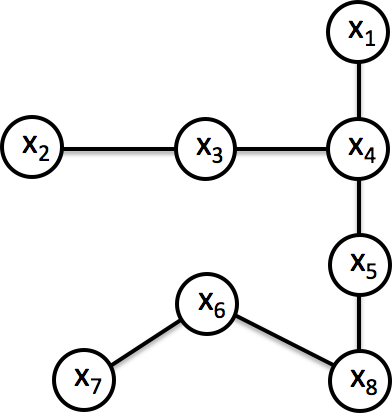
\includegraphics[height=4cm]{img/neurontree.png}}
	\end{minipage}
	\begin{minipage}[b]{0.49\linewidth}
		\centerline{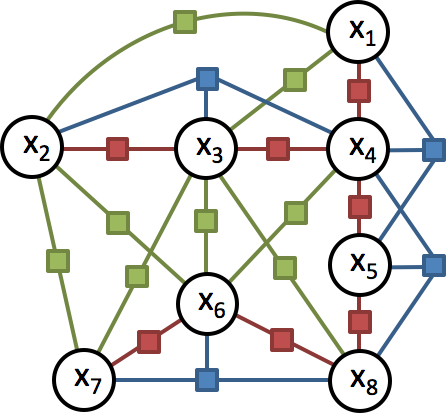
\includegraphics[height=4cm]{img/neuronmrf.png}}
	\end{minipage}
	\vspace{-10pt}
	\caption{\small{shows the tree structure or pictorial structure of the neuron (left) and our corresponding graphical model (right). Red cliques $\mathcal{E}_R$ form the tree structure of neuron. Green cliques $\mathcal{E}_G$ represent the repulsive edges, and blue cliques are the tertiary potential. Some of green and blue cliques were left out for the sake of visualization.}}
	\label{fig:sample_frame}
	\vspace{-10pt}
\end{figure}


\subsection{Unary Potential} \label{sec:unary_pot}
The data penalty term or unary potential assigns the position of the centerline based on the image appearance and the initial neuron's shape. It composes of image feature and dynamics model terms.
\begin{equation}
A\left( {\bf x}_i^t | {\bf I}, {\bf S}^0 \right) = A_{img}\left({\bf x}_i^t | {\bf I}\right) + A_{model}\left({\bf x}_i^t | {\bf I}, {\bf S}^0\right)
\end{equation}

{\bf Image feature} assigns the position of node ${\bf x}_i^t$ based on the response from the Frangi filter \cite{Frangi1998} for dendrites and the Hessian-based function for branch points. Frangi filter is a vesselness-filter designed to detect only the line-like structure, so a different function is required for the branch point (fig.~\ref{fig:vesselness}). In 2D, the branch point appears like a blob so we design a function similar to Frangi filter that has high value only when both eigenvalues of Hessian matrix are high.
\begin{equation} \label{eq:vesselness}
A_{img}\left({\bf x}_i^t | {\bf I}\right) =
\begin{cases}
\exp \left( -\frac{R_B^2}{2\beta^2} \right) \left(1-\exp \left( -\frac{S^2}{2c^2} \right) \right) &, \mbox{if } deg({\bf x}_i^t) \le 2 \\
\left( 1-\exp \left( -\frac{R_A}{2\beta^2} \right) \right) \left(1-\exp \left( -\frac{S^2}{2c^2} \right) \right) &, \mbox{otherwise}\\
\end{cases}
\end{equation}
where $deg({\bf x}_i^t)$ is the degree of the node ${\bf x}_i^t$, which is less than or equal to two if they are dendrite nodes, otherwise, they are branch points or joints between dendrites. $R_B = \lambda_1/\lambda_2$ is the ratio accounts for the deviation from a blob-like to a line-like structures, where $\lambda_k$ is the eigenvalue of the Hessian matrix at position ${\bf x}_i^t$ with the k-th smallest magnitude. $R_A = \sqrt{min(\lambda_1,0) \cdot min(\lambda_2,0)}$ measures the blob-like structure similarity for bright object over dark background, which is the branch point. For bright neurite over dark background, eigenvalues have negative values. $\lambda_1$ has low magnitude while $\lambda_2$ has high magnitude over lines. On the other hand, both eigenvalues have high magnitude at branch points. $S = \lambda_1^2 + \lambda_2^2$ distinguishes the neurite from the background since noises produce eigenvalues with low magnitude. $\beta$ and $c$ are parameters controlling the sensitivity of $R_A$, $R_B$, and $S$ \cite{Frangi1998}.

\begin{figure}[b!]
	\centering
	\begin{minipage}[b]{0.22\linewidth}
		\centerline{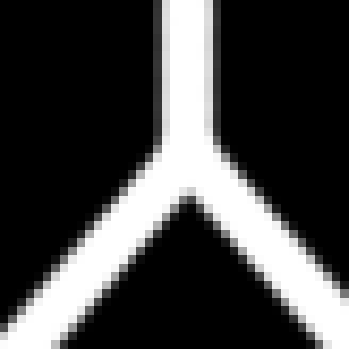
\includegraphics[height=2.5cm]{img/branch.png}}
	\end{minipage}
	\begin{minipage}[b]{0.22\linewidth}
		\centerline{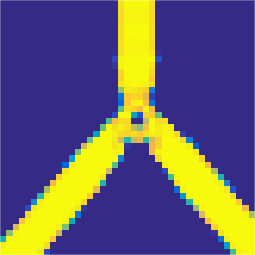
\includegraphics[height=2.5cm]{img/branch_frangi.png}}
	\end{minipage}
	\begin{minipage}[b]{0.22\linewidth}
		\centerline{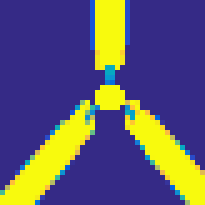
\includegraphics[height=2.5cm]{img/branch_hessian.png}}
	\end{minipage}
	\hspace{-10pt}
	\begin{minipage}[b]{0.08\linewidth}
		\centerline{
\includegraphics[height=2cm]{img/colorbar.png}}
		\vspace{7pt}
	\end{minipage}
	\vspace{-10pt}
	\caption{\small{shows the synthetic image of a branch point (left) with its corresponding Frangi filter (middle) and our Hessian-based function (right) from eq.~\ref{eq:vesselness}. Frangi filter gives low response at the center of the branch point while our Hessian-based function gives high response at the branch point and low value to surroundings. }}
	\label{fig:vesselness}
	\vspace{-10pt}
\end{figure}

{\bf Dynamics model} assigns the position of node ${\bf x}_i^t$ such that the node's position resembles to its position from our motion model, which is governed by the soma's location. Pairwise and tertiary potentials ensure that tracked neurons inherit shape characteristics of neurons, and they depend on the image feature to guide a neuron trace to the correct position. Image feature alone is not enough to locate dendrites because the whole dendrites can disappear in some frames of calcium images. The dynamics model solves this problem by introducing the motion model or the initial guess of the centerline location, which can be seen as the prior, to complement the image feature. Although dendrites are difficult to detect, on the other hand, the soma is very clear and easy to locate. In this work, we assume ${\bf S}^0$ is given, then our motion model is obtained by shifting the initial trace so that the locations of soma agree,
\begin{equation} \label{eq:dynamic}
A_{model}\left({\bf x}_i^t | {\bf I}, {\bf S}^0\right) = \exp \left( \alpha_d \cdot \left\| {\bf x}_i^t - T_{0,t}({\bf x}_i^0) \right\| \right)
\end{equation}
where $\|\cdot\|$ is the Euclidean distance. $\alpha_d$ is the parameter with negative value that tunes the sensitivity of the dynamics model. $T_{t_1,t_2}$ is the translation operator that shifts the soma's position at time $t_1$ to its position at time $t_2$, so $T_{t_1,t_2} = \sum_{t=t_1+1}^{t_2} {\bf v}_0^t$, where ${\bf v}_0^t = {\bf x}_0^t - {\bf x}_0^{t-1}$ and ${\bf x}_0^t$ are the mapping vector and position of the soma at time $t$, respectively. The positions of the soma is located by the Circle Hough Transform technique \cite{Duda1972, Atherton1999} and tracked along the optical flow computed by the FullFlow method \cite{Chen2016}.

\subsection{Pairwise Potential} \label{sec:pairwise_pot}
The pairwise smoothness assigns the position of node such that the mapping function is smooth and the transformed neuron maintains the global shape. It consists of the transition similarity and the part-based model energies. These two types of energies applied on two different types of edges, $\mathcal{E}_R$ and $\mathcal{E}_G$. It is defined as,
\begin{equation} \label{eq:pairwise}
I\left({\bf x}_i^t,{\bf x}_j^t | {\bf S}^{t-1}\right) =
\begin{cases}
\alpha_p \cdot \exp \left( \alpha_t \cdot \| {\bf v}_i^t - {\bf v}_j^t \| \right) 
&, \mbox{if } e_{ij} \in \mathcal{E}_R \\
\left[ \left\| {\bf x}_i^t - {\bf x}_j^t \right\| > \left\langle \left\| {\bf x}_k^t - {\bf x}_l^t) \right\| \right\rangle_{e_{kl} \in \mathcal{E}_R} \right]
&, \mbox{if } e_{ij} \in \mathcal{E}_G \mbox{ and } \\
& br({\bf x}_i^t) \neq br({\bf x}_j^t) \\
0 &, \mbox{otherwise}
\end{cases}
\end{equation}
where $[\cdot]$ is the indicator function taking value 1 if a given predicate is true, otherwise, value 0. $\langle \cdot \rangle$ is the expectation value. $br({\bf x}_i^t)$ is the branch number in which the node ${\bf x}_i^t$ is. $\alpha_p = \left( 2 \left\langle \left\| {\bf v}_i^t - {\bf v}_j^t \right\| \right\rangle \right)^{-1}$ is the parameter that ensures this term to scale properly between small and large vector difference \cite{Boykov2001b}, while $\alpha_t$ scales the sensitivity of the exponential term.

{\bf Transition similarity} enforces the smoothness of mapping vectors between adjacent nodes. It is applied over tree structure edges $e_{ij} \in \mathcal{E}_R$. It is defined by the function of the mapping vector difference between adjacent nodes so it encourages adjacent nodes to have the same or similar mapping vector.

{\bf Part-based model} constrains the morphology of the neuron structure using the repulsive edges \cite{Ferrari2009}. It makes dendrites to repel each other and prevents them from creating any unnecessary crossover and deforming the morphology of tracked neuron. Repulsive edges $\mathcal{E}_G$ are added between nodes from different branches. They give higher energy when dendrites overlap than when they don'’t. In this work, it is computed by thresholding the distance between branches.

\subsection{Tertiary Potential} \label{sec:tertiary_pot}
The tertiary smoothness incorporates the neuron shape characteristics into the model. It is decomposed into pairwise terms so the efficient inference method can be applied.

\begin{figure}[tb!]
	\centering
	\begin{minipage}[b]{0.49\linewidth}
		\centerline{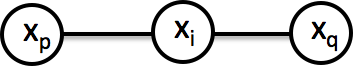
\includegraphics[width=4cm]{img/tri1.png}}
	\end{minipage}
	\begin{minipage}[b]{0.49\linewidth}
		\centerline{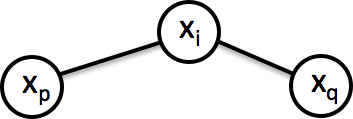
\includegraphics[width=4cm]{img/tri2.png}}
	\end{minipage}
	\vspace{-10pt}
	\caption{\small{shows that although the curvature and our decomposition are different, they share the same optimum when $\overline{{\bf x}_p^t {\bf x}_q^t} = \overline{{\bf x}_p^t {\bf x}_i^t} + \overline{{\bf x}_i^t {\bf x}_q^t}$ (left). They discourage the dendrite from bending when $\overline{{\bf x}_p^t {\bf x}_q^t} < \overline{{\bf x}_p^t {\bf x}_i^t} + \overline{{\bf x}_i^t {\bf x}_q^t}$ (right).}}
	\label{fig:triangle}
	\vspace{-10pt}
\end{figure}

{\bf Shape smoothness} ensures the smoothness of dendrites by encouraging low curvature and short length like in the active contour model \cite{Kass1988}. Computing curvature requires the tertiary potential,
\begin{equation} \label{eq:curvature}
H({\bf x}_p^t,{\bf x}_i^t,{\bf x}_q^t) = \left( {\bf x}_p^t - {\bf x}_i^t \right)^2 + \left( {\bf x}_p^t - 2{\bf x}_i^t + {\bf x}_q^t \right)^2
\end{equation}
The method in \cite{Woodford2009} decomposed the second derivative term into pairwise terms with an auxiliary node. We avoid adding auxiliary nodes by simplifying the curvature using the triangle inequality, where the clique of three nodes $\{ {\bf x}_p^t,{\bf x}_i^t,{\bf x}_q^t \}$ is decomposed into three pairwise cliques with no extra auxiliary nodes - $\{ {\bf x}_p^t,{\bf x}_i^t \}$, $\{ {\bf x}_i^t,{\bf x}_q^t \}$, and $\{ {\bf x}_p^t,{\bf x}_q^t \}$. Consider a triangle whose corners are defined by nodes ${\bf x}_p^t$, ${\bf x}_i^t$, and ${\bf x}_q^t$. The optimized curvature value is obtained when the triangle forms the straight line, $\overline{{\bf x}_p^t {\bf x}_q^t} = \overline{{\bf x}_p^t {\bf x}_i^t} + \overline{{\bf x}_i^t {\bf x}_q^t}$, so the simplification has the same optimum as the potential in eq.~\ref{eq:curvature} (fig.~\ref{fig:triangle}), which is defined as,
\begin{equation} \label{eq:H}
H({\bf x}_p^t,{\bf x}_i^t,{\bf x}_q^t) = \quad \alpha_s \cdot \left\{ \| {\bf x}_p^t - {\bf x}_i^t \|^2 + \| {\bf x}_i^t - {\bf x}_q^t \|^2 - \frac{ \| {\bf x}_p^t - {\bf x}_q^t \|^2 }{4} \right\}
\end{equation}
where $\alpha_s$ is the parameter with negative value that tunes the sensitivity of the shape smoothness. The quadratic terms encourage the short distance between nodes. This term encourages both rigidity and elasticity like the active contour model \cite{Kass1988}. The third term of the decomposition is divided by 4 to ensures that $H({\bf x}_p^t,{\bf x}_i^t,{\bf x}_q^t) \leq 0$ (the proof in appendix~\ref{sec:appA}).

\section{Implementation}
The position of centerline ${\bf X}^t$ is discretized so the problem becomes feasible. Algorithm~\ref{alg:track} shows the summary of our method given the image sequence ${\bf I}$ and the neuron trace initialization ${\bf S}^0$. In line~\ref{alg:track:optimize}, our energy function in eq.~\ref{eq:objfunc} is non-submodular so MRF is optimized using the $\alpha$-expansion \cite{Boykov2001} with QPBO \cite{Boros2002, Kolmogorov2007}, also known as fusion moves \cite{Lempitsky2010}. 

\begin{algorithm}
	\caption{Neuron tracking} \label{alg:track}
	\begin{algorithmic}[1]
		\Procedure{tracking}{ ${\bf I}$, ${\bf S}^0$ }
		\For{$t = 1$ to $\mathrm{T}$}
		\State Compute $A\left( {\bf x}_i^t | {\bf I}, {\bf S}^0 \right)$ using eq.~\ref{eq:vesselness} and~\ref{eq:dynamic}
		\State Compute $I\left({\bf x}_i^t,{\bf x}_j^t | {\bf S}^{t-1}\right)$ using eq.~\ref{eq:pairwise}
		\State Compute $H\left({\bf x}_p^t,{\bf x}_i^t,{\bf x}_q^t\right)$ using eq.~\ref{eq:H}
		\State ${\bf S}^t \gets \argmax_{{\bf X}^t} P \left( {\bf X}^t | {\bf I}, {\bf S}^{t-1}, {\bf S}^0 \right)$ \label{alg:track:optimize}
		\EndFor
		\State \Return {\bf S}
		\EndProcedure
	\end{algorithmic}
\end{algorithm}

For efficiency, the search space is limited by reducing the number of candidate positions and pruning the redundant edges from the graphical model ${\bf S}^t$.

To limit the number of candidate positions, we ignore locations that are far away from the neuron and consider only the regions around the starting location (in our experiment, within 20 pixels), which indicates the possible position based on previous trace. In this work, the starting location of each node at time $t$ is computed by applying the translation operator that shifts soma's location from previous time-step to the current position, $\widetilde{\bf x}^t_i = T_{t-1,t}({\bf x}^{t-1}_i)$. Then, the possible configuration of node ${\bf x}^t_i$ is limited to regions around the starting location $\widetilde{\bf x}^t_i$.

Redundant edges are repulsive edges linking nodes from the same branch or nodes that are far apart. They link nodes that are unlikely to overlap so removing these edges makes no difference to the model. To remove these edges, ${\bf S}^t$ is pruned such that there is at most one edge between a node and a branch, where the shortest edge is selected. Other nodes are considered far apart and edges incident to those nodes are redundant. With this scheme, we limit the number of repulsive edges $| \mathcal{E}_G | = \mathcal{O}(N)$. The total the number of edges in our model is also $\mathcal{O}(N)$ since $| \mathcal{E}_R | = \mathcal{O}(N)$ due to the tree structure of the neuron and the number of tertiary cliques is limited to three per node if every bifurcation has only two children \cite{Farhand2016}.

\section{Experiments}
% need more details about dataset from Liping He and Tracy Dan.
In this section, we apply our method on time-lapse calcium images. In this dataset, each sequence captures a few motions of neurons and the duration of each motion is around 10-20 frames. The ground truth was produced by tracing neurons manually in some frames of the image sequences, especially when there are movements over neurons. The manual reconstructions of neurons were produced using the software called \emph{neuTube} \cite{Feng2015}. Three dissimilarity metrics were used in this work, which are the spatial distance (SD), substantial SD (SSD), and the percentage of sample points used in SSD (\%SSD). SD(A,B) is defined by the mean of the average Euclidean distance of nodes in A to the closest point in B and the other way round. Nodes in A and B are resampled such that the distance between adjacent nodes is one voxel to remove the bias from trace node sampling. When most parts of neurons overlap, SD gives low values and offsets parts of the neuron that are totally out-of-place. To emphasize the magnitude of errors, SSD is defined as the SD over nodes that are apart from the other neuron at least 2 voxels. The last metric is the percentage of nodes that are apart from the other neuron. It indicates the inconsistency between two neurons. The detailed definition of these criteria is given in \cite{Peng2010}. We compared our method with the optical-flow-based neuron tracking computed by the FullFlow method \cite{Chen2016}. The experiment was carried out on Mac Pro (2$\times$2.66 GHz 6-Core Intel Xeon, 20GB 1333MHz DDR3 ECC); the run time of our method was around one second per frame per neuron. The dimension of each frame is around 512$\times$192 pixel. Tracking was done on 2D maximum projection of 3D images, albeit the availability of image stack sequences, to eliminate the color bleach effect that is more likely to occur over Z-axis due to image acquisition process, where image slices were taken in sequence.

\begin{figure*}[t!]
	\hspace{-30pt}
	\begin{tabular}{cccccc} 
		\footnotesize{Ground truth} & \footnotesize{Our model} & \footnotesize{Dynamics} & \footnotesize{Transition} & \footnotesize{Part-based} & \footnotesize{Shape} \vspace{-2pt} \\
		{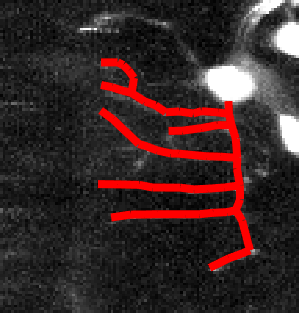
\includegraphics[width=2cm]{img/gt_t1.png}} &
		{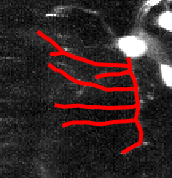
\includegraphics[width=2cm]{img/all_t1.png}} &
		{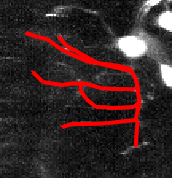
\includegraphics[width=2cm]{img/dyna_t1.png}} &
		{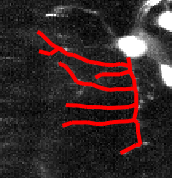
\includegraphics[width=2cm]{img/tran_t1.png}} &  
		{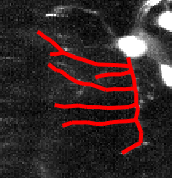
\includegraphics[width=2cm]{img/repul_t1.png}} &  
		{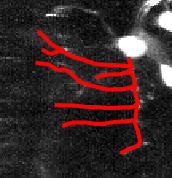
\includegraphics[width=2cm]{img/shape_t1.png}}  \\
		{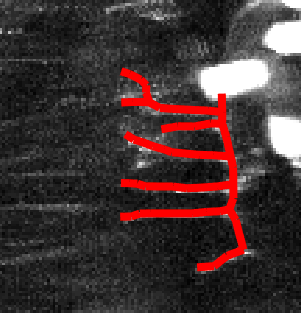
\includegraphics[width=2cm]{img/gt_t2.png}} &
		{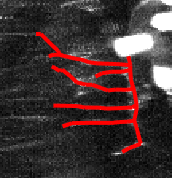
\includegraphics[width=2cm]{img/all_t2.png}} &
		{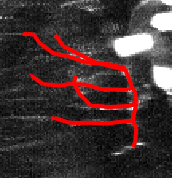
\includegraphics[width=2cm]{img/dyna_t2.png}} &
		{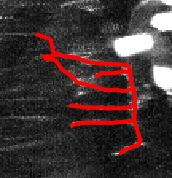
\includegraphics[width=2cm]{img/tran_t2.png}} &  
		{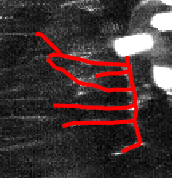
\includegraphics[width=2cm]{img/repul_t2.png}} &  
		{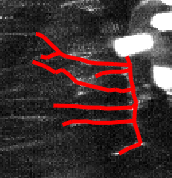
\includegraphics[width=2cm]{img/shape_t2.png}}  \\
		{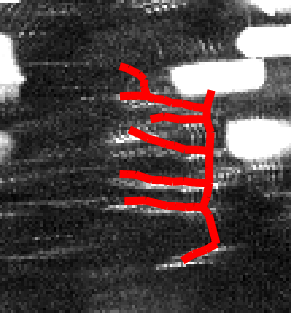
\includegraphics[width=2cm]{img/gt_t3.png}} &
		{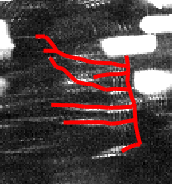
\includegraphics[width=2cm]{img/all_t3.png}} &
		{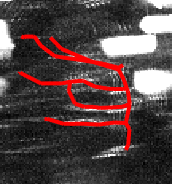
\includegraphics[width=2cm]{img/dyna_t3.png}} &
		{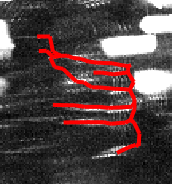
\includegraphics[width=2cm]{img/tran_t3.png}} &  
		{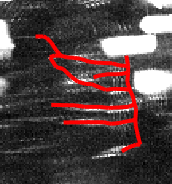
\includegraphics[width=2cm]{img/repul_t3.png}} &  
		{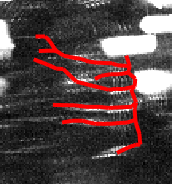
\includegraphics[width=2cm]{img/shape_t3.png}}  \\
	\end{tabular}
	\vspace{-10pt}
	\caption{\small{Tracking results (in red color) on 3 adjacent frames in each row. The first and second columns show the ground truth and our results, while the next four columns are our results excluding one of the factors - dynamics model, transition similarity, part-based model, and shape smoothness respectively. }}
	\label{fig:factors}
	\vspace{-10pt}
\end{figure*}
Fig.~\ref{fig:factors} shows the importance and effects of each factor, we display the tracking results when all factors are integrated and when one of the factors is excluded. Dynamics model is required to compensate for the unreliability of image intensity. Without this factor, nodes move towards the pixel with high intensity regardless of neuron's shape. Transition similarity prevents rapid changes in adjacent nodes resulting in smooth mapping. Part-based model ensures dendrites avoid overlapping. Finally, shape smoothness smooths out the dendrites; otherwise, crooked curves are detected due to dip in intensity over neurites. 

\begin{figure}[tb!]
	\centering
	\begin{minipage}[b]{0.67\linewidth}
		\centerline{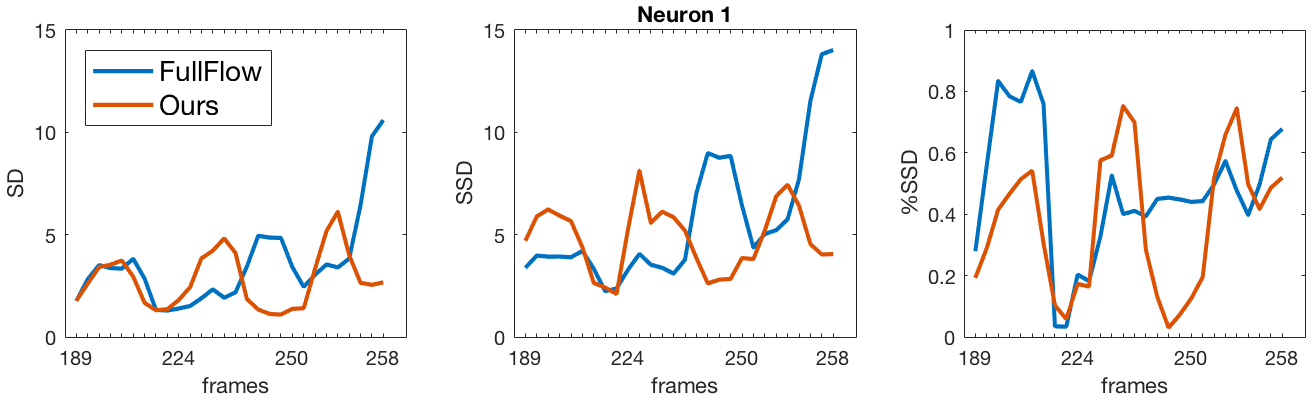
\includegraphics[width=\linewidth]{img/neuron1stat.png}}
	\end{minipage}\\
	\begin{minipage}[b]{0.67\linewidth}
		\centerline{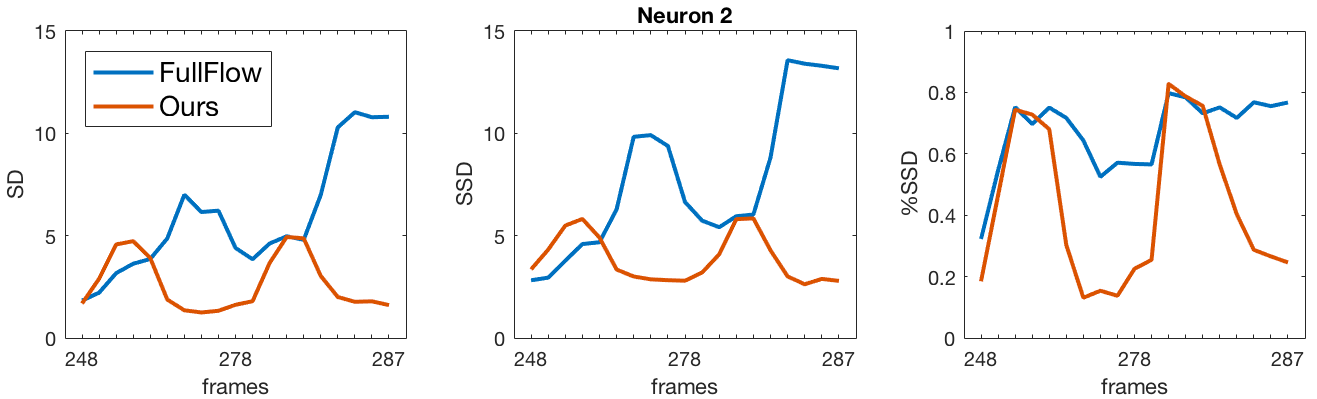
\includegraphics[width=\linewidth]{img/neuron2stat.png}}
	\end{minipage}
	\vspace{-10pt}
	\caption{\small{shows three dissimilarity scores - SD, SSD, and \%SSD, of FullFlow \cite{Chen2016} and our method. Rows display the tracking results of two different neurons. The first row shows the easy case where the SNR is high. The second row shows the difficult case where the SNR is low.}}
	\label{fig:neuronstat}
	\vspace{-10pt}
\end{figure}
We evaluate our method and competitor using the dissimilarity criteria on image sequences with low and high signal-to-noise ratio (SNR) to illustrate the advantage of our method in fig.~\ref{fig:neuronstat} and~\ref{fig:neuronboxplot}. For each frame, three scores are computed on our results and competitor's (fig.~\ref{fig:neuronstat}). They show that our method gives high error when neurons move, especially \%SSD that peaks at the middle of the motions. The error arises from the out-of-focus problem because the imaging system acquires blurry images when the organism moves, as well as the neuron. Another advantage is that even though our method may produce wrong tracked neuron, the distance error from the ground truth is low as shown by SSD scores, which is around 5 pixels on the testing data.

To get the summary of performance, the box plot of SD score is displayed in fig.~\ref{fig:neuronboxplot}. It shows that our results are comparable to the competitor when SNR is high but our results outperforms the other method when SNR is low. This observation is supported by the qualitative results in fig.~\ref{fig:neuroncompare}. It illustrates that optical-flow-based method fails to recover the motion field, resulting in poor tracked neuron centerline. While our method integrates shape and motion information with intensity to produce the robust tracking results.
\begin{figure}[b!]
	\centering
	\begin{minipage}[b]{0.25\linewidth}
		\centerline{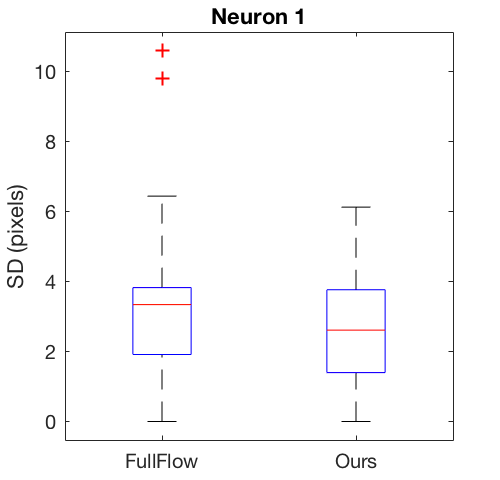
\includegraphics[width=\linewidth]{img/box_n1.png}}
	\end{minipage}
	\begin{minipage}[b]{0.25\linewidth}
		\centerline{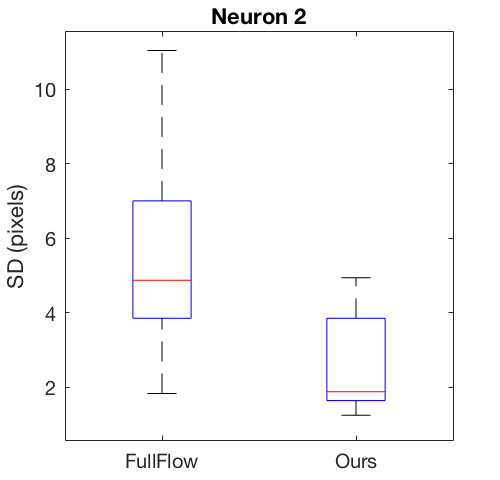
\includegraphics[width=\linewidth]{img/box_n2.png}}
	\end{minipage}
	\vspace{-10pt}
	\caption{\small{shows the box plot of SD scores produced by our method and FullFlow \cite{Chen2016} when SNR is high (left) and low (right). In a box plot, the red line indicates the median. The bottom and top of the rectangle indicate the first and third quartiles respectively. The vertical line shows the range of value and outliers are plotted individually.}}
	\label{fig:neuronboxplot}
\end{figure}

\begin{figure}[tb!]
	\centering
	\begin{tabular}{ccc} 
		\footnotesize{Ground truth} & \footnotesize{FullFlow} & \footnotesize{Our model} \vspace{-2pt} \\
		{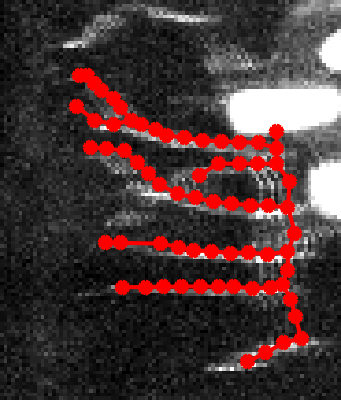
\includegraphics[width=2.5cm]{img/gt_n3a.png}} &
		{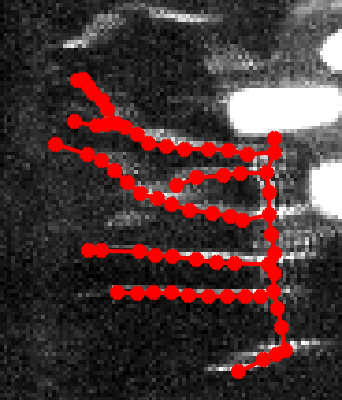
\includegraphics[width=2.5cm]{img/ff_n3a.png}} &
		{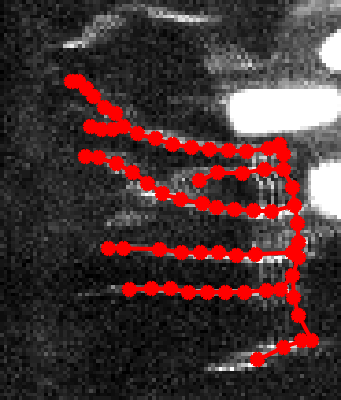
\includegraphics[width=2.5cm]{img/our_n3a.png}}  \\
		{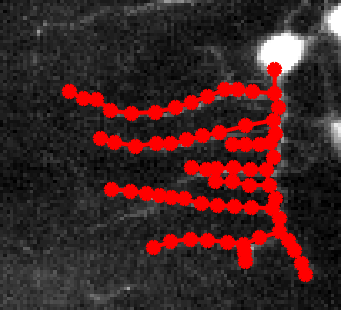
\includegraphics[width=2.5cm]{img/gt_n3b.png}} &
		{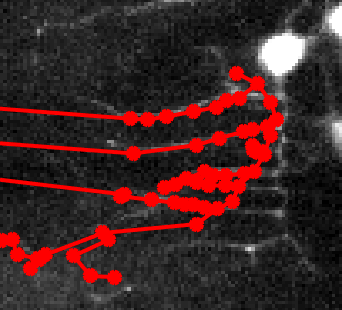
\includegraphics[width=2.5cm]{img/ff_n3b.png}} &
		{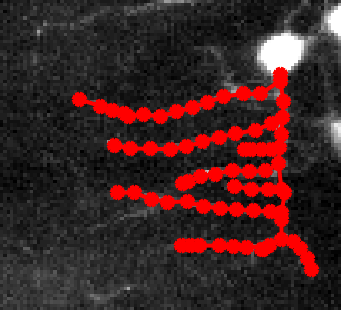
\includegraphics[width=2.5cm]{img/our_n3b.png}}  \\
	\end{tabular}
	\vspace{-10pt}
	\caption{\small{shows the ground truth (left), results from FullFlow (middle), and our results (right) in red color. Rows show tracking results when SNR is high (top) and low (bottom).}}
	\label{fig:neuroncompare}
\end{figure}

% References should be produced using the bibtex program from suitable
% BiBTeX files (here: strings, refs, manuals). The IEEEbib.bst bibliography
% style file from IEEE produces unsorted bibliography list.
% -------------------------------------------------------------------------
\bibliographystyle{IEEEbib}
\small{\bibliography{refs}}

\appendix
\section{Appendix A} \label{sec:appA}
Here we prove that $H({\bf x}_p^t,{\bf x}_i^t,{\bf x}_q^t) \leq 0$ (eq.~\ref{eq:H}). From the triangle inequality,
\[
\begin{aligned}
\| {\bf x}_p^t - {\bf x}_i^t \| + \| {\bf x}_i^t - {\bf x}_q^t \| & \geq \| {\bf x}_p^t - {\bf x}_q^t \| \\
(\| {\bf x}_p^t - {\bf x}_i^t \| + \| {\bf x}_i^t - {\bf x}_q^t \|)^2 & \geq \| {\bf x}_p^t - {\bf x}_q^t \|^2 \\
\end{aligned}
\]
Let $a = \max\{ \| {\bf x}_p^t - {\bf x}_i^t \|, \| {\bf x}_i^t - {\bf x}_q^t \| \}$, then
\[
\begin{aligned}
(2a)^2 & \geq \| {\bf x}_p^t - {\bf x}_q^t \|^2 \\
a^2 & \geq \frac{\| {\bf x}_p^t - {\bf x}_q^t \|^2}{4} \\
\| {\bf x}_p^t - {\bf x}_i^t \|^2 + \| {\bf x}_i^t - {\bf x}_q^t \|^2 & \geq \frac{\| {\bf x}_p^t - {\bf x}_q^t \|^2}{4} \\
\end{aligned}
\]
$\alpha_s$ has negative value so $H({\bf x}_p^t,{\bf x}_i^t,{\bf x}_q^t) \leq 0$.
\end{document}
